\documentclass{sig-alternate}

\usepackage{times}
\usepackage{verbatim}
\usepackage{subfigure}
\usepackage{multirow}
\usepackage{url}
\usepackage{color}
\usepackage{balance}
\makeatletter
\newif\if@restonecol
\makeatother
\let\algorithm\relax
\let\endalgorithm\relax
\usepackage[lined,algonl,boxed]{algorithm2e}%\usepackage{mathbb}

\newcommand{\reminder}[1]{\textbf{\color{red}[** #1 **]}}  % to fix
\newcommand{\hide}[1]{} %hide
\newcommand{\vpara}[1]{\vspace{0.08in}\noindent\textbf{#1 }}
\newcommand{\para}[1]{\vspace{0.01in}\noindent\textbf{#1 }}
\newcommand{\secref}[1]{Section~\ref{#1}} %section reference
\newcommand{\Real}{\ensuremath{\mathbb{R}}}  % Real numbers
\newcommand{\figref}[1]{Figure~\ref{#1}} %section reference
\newcommand{\beq}[1]{\vspace{-0.02in}\begin{equation}#1\end{equation}\vspace{-0.02in}}
\newcommand{\beqn}[1]{\vspace{-0.03in}\begin{eqnarray}#1\end{eqnarray}\vspace{-0.03in}}
\newcommand{\beal}[1]{\vspace{-0.03in}\begin{align}#1\end{align}\vspace{-0.03in}}
\newcommand{\besp}[1]{\begin{split}#1\end{split}}
\newcommand{\remark}[1]{\textbf{\color{red}**#1**}}
%\newcommand{\eeq}[1]{\end{equation}\normalsize}

\newdef{definition}{Definition}
\newdef{problem}{Problem}
\newdef{theorem}{Theorem}
\newtheorem{hypothesis}{Hypothesis}

\newfont{\mycrnotice}{ptmr8t at 7pt}
\newfont{\myconfname}{ptmri8t at 7pt}
\let\crnotice\mycrnotice%
\let\confname\myconfname%


\begin{document}

\title{Null Models For Social Networks}

\numberofauthors{2}
%
% Put no more than the first THREE authors in the \author command

% NOTE: All authors should be on the first page. For instructions
% for more than 3 authors, see:
% http://www.acm.org/sigs/pubs/proceed/sigfaq.htm#a18
\author{
%
% The command \alignauthor (no curly braces needed) should
% precede each author name, affiliation/snail-mail address and
% e-mail address. Additionally, tag each line of
% affiliation/address with \affaddr, and tag the
%% e-mail address with \email.
\alignauthor Jessica Su\\
       \affaddr{Department of Computer Science}\\
       \affaddr{Stanford University}\\
       \email{jtysu@stanford.edu}
\alignauthor Sen Wu\\
       \affaddr{Department of Computer Science}\\
       \affaddr{Stanford University}\\
       \email{senwu@stanford.edu}
}

\maketitle
\begin{abstract}

%Networks with similar motif distributions tend to have similar functions in the real world~\cite{chuanqi}.

In this paper, we present a heuristic method to generate graphs with specific motif counts.  Motif counts imply many structural properties of a graph, such as clustering coefficient and degree distribution (Section~\ref{sec:alpha}), and can be used to cluster networks into meaningful real-world categories~\cite{chuanqi}.  By constructing graphs with specific motif counts, we hope to build models that will imitate the functionality of specific networks.

Our method is based on hill-climbing.  We perform successive transformations on an initial graph, keeping the ones that reduce error and discarding the ones that don't.  Running this algorithm on $9$ real-world networks shows substantial improvement over the baseline.  On our metabolic network, our model's motif counts were identical to the motif counts of the original network.  On our power grid network, the average relative error between the motif counts of our model and the network was $0.006$.  All networks saw at least a 58\% decrease in average relative error, with most networks seeing much better performance.

%Social motif has widely used for clustering large social network. However, graph generation algorithms often focus on degree distribution and lack of motif distribution. In this paper, we define the motif-driven graph generation problem and present a heuristic method which focus constructing the approximate motif distribution of large network. Our experiments on 67 real social network motif network distribution show that our approach obtains the generated graph with similar motif distribution within relevant error less then 0.02 in 10 hours.

\end{abstract} 

%\vspace{-0.02in}
% A category with only the three required fields
\category{J.4}{Social and Behavioral Sciences}{Miscellaneous}

%\category{H.4.m}{Information Systems}{Miscellaneous}
%\vspace{-0.08in}
\terms{Algorithms, Experimentation}
%\vspace{-0.08in}
\keywords{Social networks}


\section{Introduction}
\label{sec:intro}

Many real-world systems can be modeled by graphs, from power grids to arXiv citations to friendships on Facebook.  Early models attempted to model all systems with the same type of graph.  For example, the Erdos-Renyi random graph~\cite{erdds1959random}\cite{erdos1960random} models all networks with $n$ participants and $m$ connections with a graph of $n$ nodes and $m$ randomly placed edges.  The Watts-Strogatz model~\cite{watts1998collective} models all networks by connecting nodes to their nearest neighbors, then filling the rest of the graph with randomly placed edges.

More sophisticated models account for differences in degree distribution and clustering coefficient.  The preferential-attachment model~\cite{albert2002statistical} generates a graph with power-law degree distribution and allows the modeler to choose the exponent in the power law.  The configuration model takes as input an exact sequence of degrees and creates a random graph with that degree sequence.  Newman's "triangle-edge" model~\cite{newman2009random} generalizes this to create a random graph with specific degree sequence and clustering coefficient.

In our model we create a random graph with specific degree sequence and motif counts.  Algorithms that classify social networks according to their motif counts find clusters that correspond closely to real-life functionality~\cite{chuanqi}.  Therefore, by generating graphs with similar motif counts, we hope to build graphs that function similarly to real-life social networks.

While it is difficult to find exact solutions, we use hill-climbing to find approximate solutions that produce good results in practice.
\section{Background}
\label{sec:background}

\begin{figure}[t]
\centering
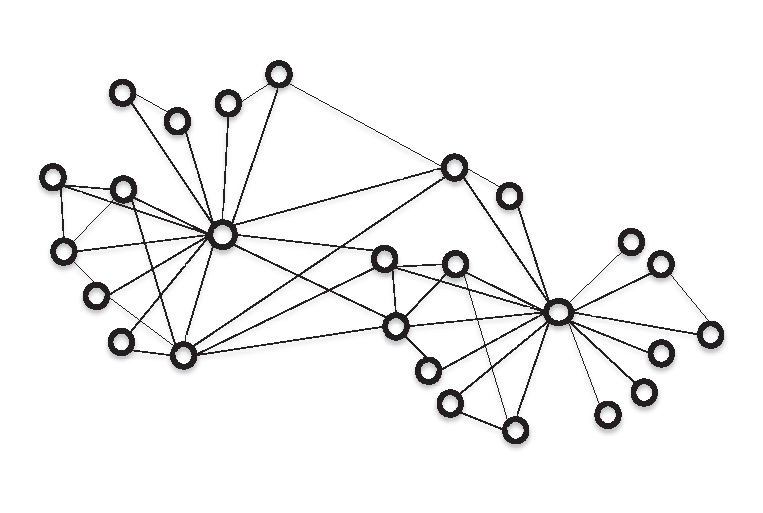
\includegraphics[width=3in]{Figures/network.eps}
\caption{A sample social network.}
\label{fig:network}
\end{figure}

\begin{figure}[t]
\centering
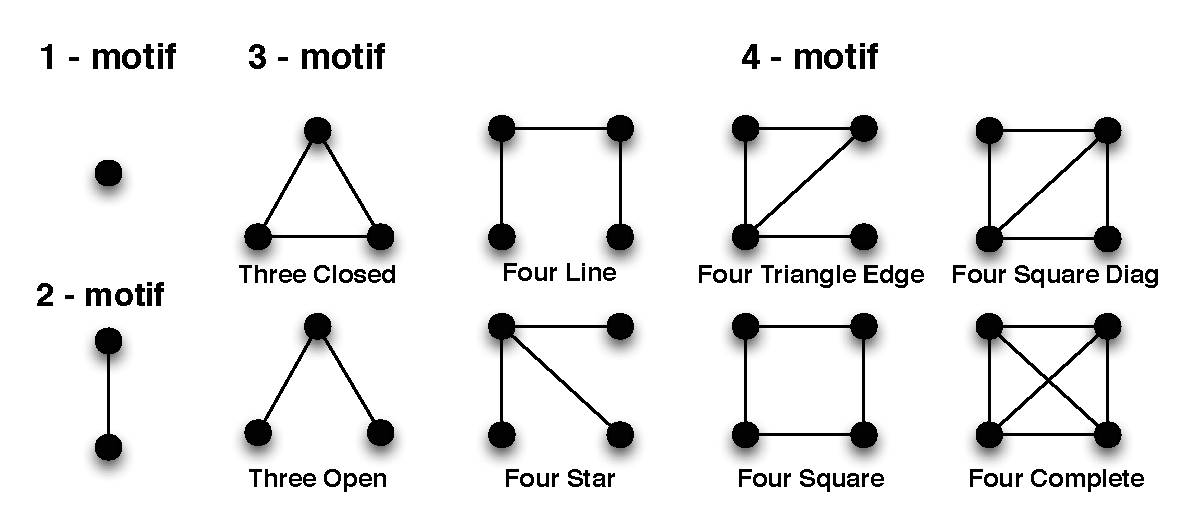
\includegraphics[width=3in]{Figures/motifs1.eps}
\caption{Graphical representation of the motifs.}
\label{fig:motif}
\end{figure}

In this section, we first give some basic concepts that we use throughout the paper. Then, we formulate the problem of motif-driven graph generation. 

%A \textbf{graph} is a representation of a set of objects and the
%connections between them.  It is defined as a tuple $(V, E)$, where $V$ is
%a set of $|V| = N$ vertices ("nodes") and $E \subseteq V \times V$ is a set of edges.
%The nodes in a graph correspond to the objects, and the edges to
%the connections.
%
%A graph is called \textbf{simple} if no node has an edge to itself and no two
%nodes have more than one edge between them.  A graph is \textbf{undirected}
%if whenever $(v, w)$ is an edge, $(w, v)$ is also an edge.  In our problem, 
%we assume all graphs are simple and undirected.
%
%A \textbf{subgraph} of $G$ is a graph whose nodes and edges form subsets of 
%the nodes and edges of the graph $G$.  An
%\textbf{induced subgraph} of $G$ on the vertices $V' \subseteq V$ is the
%graph consisting of the vertices $V'$ and the edges between them.

A \textbf{motif} is a small, connected graph, often considered as a
subgraph of a larger graph. In this paper, we only
consider motifs with at most $4$ vertices, which we term "1-motif", "2-motif", "3-motif" and
"4-motif" respectively. Note that a 1-motif is simply a vertex, and a 2-motif is simply an edge. A full list of motifs is shown in
Figure~\ref{fig:motif}.

The \textbf{motif distribution} of a graph $G$ specifies how many of each
motif type the graph contains.  For example, the graph in Figure~\ref{fig:network} has motif
distribution \{numNodes: 25, numEdges: 44, mtThreeClosed: 21, mtThreeOpen: 151, mfFourLine: 134,
mfFourSquare: 1, mfFourStar: 305, mfFourTriangleEdge: 155, mfFourSquareDiag:
26, mfFourComplete: 2\}.  This graph contains 25 nodes, 44 edges, 21 triangles, two 4-cliques, and
so forth.

\section{Problem Definition}
\label{sec:problem}
\vpara{Problem:} To generate a network with desired specifications.

\vpara{Input:} The input of our problem consists of is the motif 
distribution $D$. In this paper, we only consider motif within 4 vertices.

\vpara{Output:} Our goal is to generate a graph $G$ which has motif distribution that closely
approximates $D$.

Ideally we would generate a graph with the exact motif distribution $D$.
In the next section we show that problem is NP-hard, so the best we can 
hope for is an approximation.

The problem formulation is different from other graph generation problems
\cite{erdds1959random, watts1998collective, albert2002statistical,
newman2009random, molloy1995critical}, as in this paper we focus on
generating graphs based on the motif distribution.
Motif distributions are frequently used for analyzing large graphs in the
social sciences.

\section{Hardness of Problem}
\label{sec:nphard}

In this section, we describe the difficulty of the exact motif generation problem.


Given the definition of problem, the motif-driven graph generation problem can be cast as nonlinear programming problem. Let $X_{ij}$ denote the existence of the edge $(v_i, v_j)$ in graph, where $X_{ij} = 1$ if edge $(i, j)$ is in graph, $0$ otherwise. With the motifs can be represent by a polynomial combination of $X_{ij}$, for example, Three Closed of nodes $v_a, v_b, v_c$ as $X_{ab}X_{bc}X_{ac}$ and Four Triangle Edge of $v_a, v_b, v_c, v_d$ as $X_{ab}X_{bc}X_{ca}X_{ad}(1 - X_{bd})(1 - X_{cd})$. For each kind of motif, we can build a nonlinear function to represent the number of motif. Then, we can construct a nonlinear equations.

\theorem The problem of motif generate grpah by $k$-motif is NP-hard, even in the case of there is only triangle closed motif.

\Proof In the case of triangle closed motif, the problem can be reduced to $min\{\sum_{i,j,k} X_{ij}X_{jk}X_{ki}\}, X_{ij} \in \{0, 1\}$, which is an typical nonlinear integer programming. And the problem can further equal to
\begin{align*}
\min\mbox{ }&C\\
s.t. &\sum_{i,j,k} X_{ij}X_{jk}X_{ki} \leq C\\
&X \geq 0, X \in \{0, 1\}^n
\end{align*}

According to R. Hemmecke's~\cite{hemmecke2009nonlinear} theory, $\sum_{i,j,k} X_{ij}X_{jk}X_{ki} \leq C$ can be transfer to the linear function, which means the problem equals to the a special case of  linear programming which is 0-1 integer linear programming. This problem is known to be NP-complete. This is one of Karp's 21 NP-complete problems; \cite{karp1972reducibility} Karp showed the NP-completeness by a reduction from the vertex cover problem. So, our motif generation is also NP-complete.

\section{Data and Observations}
\label{sec:observations}

\section{Our Approach}
\label{sec:approach}

In this section, we present a approach framework for generating the graph. At the high level, our proposed framework consists of two stage.
\begin{itemize}
    \item {\bf Degree distribution generation.} First, given a certain motif distribution, we train a gradient boosting model using the motif distribution. And then we predict the degree distribution from motif distribution.
    \item {\bf Candidate graph generation.} Second, with the degree distribution, we generate a random graph based on degree distribution as candidate graph for our problem.
    \item {\bf Graph refinement.} Second, the random graph is fed to a heuristic model to refine the graph. The model incorporates the several strategies to refine the graph satisfied the given motif distribution.
\end{itemize}

\subsection{Degree distribution generation} 

In order to better generate random graphs, we assume that all the graphs generated are based on power law degree distributions. The basic idea is to use the motif distribution as features to predict the degree distribution. In this paper, we use Gradient Boosted Regression Trees (GBRT)~\cite{friedman2002stochastic} as the main regression model. Gradient Boosted Regression Trees is a useful machine learning method for regression problems, which also is an ensemble method with combines multiple weak prediction models. It constructs the model in a stage-wise fashion and generalizes the model by optimizing a arbitrary differentiable loss function which in our case is the square loss function\footnote{Square Loss: $\mathcal{L} = (f(x) - y)^2$, here we use $\mathcal{L}$ to describe the squared loss term, $y$ represents the label and $f(x)$ represents the predict score.}. 

More precisely, GBRT trains several small tree regression models (the depth of each tree is 5), each with high bias. Instead of using a uniform weight for each model to prevent the overfitting, GBRT focuses on adding new trees to minimize the current remaining regression error at each iteration. Let $f(x_i)$ denote the prediction score of sample $x_i$ and $\mathcal{L}(f(x_1),...,f(x_n))$ as the loss function of the model, which reaches a minimum if $f(x_i) = y_i$ for all $x_i$. For each new tree $T_i$, that is added into the existing classifier and the current prediction $P(x_i)$, we use the following step:
$$P(x_i) \leftarrow P(x_i) + \alpha \frac{\mathcal{L}}{P(x_i)}$$
\noindent where $\alpha$ is the learning rate, and the gradient $\frac{\mathcal{L}}{P(x_i)}$ is approximated with the prediction score of regression tree~\cite{zheng2007general}. Algorithm~\ref{algo:gbrt} shows the details of GBRT.

\begin{algorithm}
\caption{Gradient Boosted Regression Trees (GBRT). DT indicates the decision tree model which has three parameters, data $D$, #features\mbox{ }f and the depth $d$ of tree.}\label{algo:gbrt}
\begin{algorithmic}
\State \textbf{Input:} Data set $\mathcal{D} =\{(x_1, y_1),..., (x_n, y_n)\}$, learning rate\mbox{ }\alpha, \#Trees\mbox{ }$M$, depth\mbox{ }$d$ \\
\State \textbf{Output:} Combined tree model T

\State Initialization: $\forall i, p_i \leftarrow y_i$

\For {$i = 1$ to $M$} {
    $T_i \leftarrow DT(\{(x_1, p_1),..., (x_n, p_n)\}, f, d)$ \\
    \For {$j = 1$ to $n$} {
        $p_i \leftarrow p_i - \alpha T_i(x_i)$\\
    }
}
$T \leftarrow \alpha \sum_{i = 1}^M T_i$\\
\Return T\\
\end{algorithmic}
\end{algorithm}

\vpara{Implement Note.} In the Decision Tree model, we train $M = 1000$ trees and for each tree tree random select $f = \#\mbox{features} / 10$ and set the depth to 5. If $M$ is too big, the algorithm starts overfitting. As for learning rate, we use $\alpha = 0.001$.


\hide{We use the motif distribution to predict the degree distribution.
For a given motif distribution, we use the motif distribution to predict degree distribution. The idea of this problem is using the motif distribution as a feature to train a model, and then predict a degree distribution for the given motif distribution. More precisely, we use gradient boosting as the main regression method to train a model. Gradient Boosting Tree~\cite{friedman2002stochastic} is a useful machine learning method for regression problems, which also an ensemble method with combine multiple weak prediction models. It makes the model in a stage-wise fashion and generalizes the model by optimization of the arbitrary differentiable loss function which is same as logistic regression. Here we use the python package build in~\cite{pedregosa2011scikit}. Our approach shows good performance. We achieved less than 1\% on Average Relative Error.
}

\vpara{Evaluation Measures} To quantitatively evaluate the performance of predicting the degree distribution, we conducted experiments with different networks. For each network, we evaluated the approaches in terms of \textbf{Average Relative Error (ARE)}.

\vpara{Prediction Performance} We use 168 different networks as input data to evaluate the proposed model, with 10-fold cross validation. In order to avoid bias, we test the data 10 times, and get the prediction alpha for each network. This model achieves \textbf{Average Relative Error (ARE)} sore $0.005521$ with standard deviation $0.00316$.

\subsection{Candidate graph generation}

According the degree distribution we got at stage 1, we use 


=======================================

In this section, we propose a heuristic method for generating the required
graph.

\subsection{Hill climbing}
Hill-climbing is a standard technique for finding good solutions to optimization problems.  Start with a solution that is not particularly good.  At each step, perturb the solution randomly.  If the new answer is better, keep it; if not, keep the old solution.  Repeat this until the algorithm converges to a good solution.

Hill-climbing does not guarantee an optimal solution, since it tends to get stuck at local maxima.  Yet in practice the solutions it finds are "pretty good," especially after running the algorithm several times and picking the best solution.

In our case we minimize the error between the desired motif counts and our solution's motif counts:
\begin{equation}
\label{eqn:avgRelativeError}
\mbox{Average relative error} = \frac{1}{\ell} \sum_{i = 1}^{\ell} \frac{|\mbox{counts}_i - \widehat{\mbox{counts}}_i| + 1}{|\mbox{counts}_i| + 1}
\end{equation}
where $\ell$ is the number of different motif types.

We use the configuration model to generate a random graph with the required degree sequence.  Then at each step we choose two edges (at random) and swap their endpoints.  We count the motifs and compare the error with the new counts to the error with the old counts.  If the new counts give a smaller error, we keep the new graph; otherwise, we discard it.

\begin{algorithm}[t]
\caption{Naive approach}
\label{algorithm:naive}
\begin{algorithmic}
Initialize graph $G = (V, E)$ with prescribed degree sequence\\
motifCounts <- CountMotifs($G$)\\
\Repeat{computation time limit exceeded} {
	Choose $e_1, e_2 \in E$ at random\\
	Add edges $(e_1.Src, e_2.Dst)$, $(e_2.Src, e_1.Dst)$\\
	Delete edges $(e_1.Src, e_1.Dst)$, $(e_2.Src, e_2.Dst)$\\
	newMotifCounts <- CountMotifs($G$)\\
	\eIf {error(newMotifCounts) < error(motifCounts)} {
		motifCounts <- newMotifCounts\\
	} {
		Return graph to original state\\
	}
}

\end{algorithmic}
\end{algorithm}

\subsection{Optimizations}
As written, this solution is very slow.  Counting motifs is $O(|V|^4)$ and takes unacceptably long in practice.  To get good results in practice, we need a large number of rewiring steps, so ideally each rewiring step should take less than a second.

We can speed this up by counting motifs incrementally.  Instead of considering the whole graph on every step, we only look at the part of the graph whose motifs would be affected by the edge changes.  Since we are only looking at motifs with fewer than $5$ nodes, we can only consider the nodes that are one or two hops away from the nodes whose edges are being rewired.  Then we can count how many motifs are being created or destroyed in the induced subgraph on those nodes, and add those to the total motif counts.  Once we have the induced subgraph, we count the motifs by taking all possible sets of four vertices, and seeing which motif they form, if any.

(In our algorithm we break the rewiring step into four steps, two edge deletions and two edge creations.  This way we only measure the effect of one edge creation/deletion step at a time.)

This is still fairly slow, so we apply one final optimization.  We notice that for a 4-motif to be affected by the edge changes, vertices $1$ and $2$ of the motif must be endpoints of the edge.  Vertex $3$ must be an immediate neighbor of an endpoint, and vertex $4$ is either an immediate neighbor or a second-degree neighbor.  Ordinarily, we would have to loop through the immediate neighbors to find all possibilities for vertex $3$, and perform an inner loop through the second degree neighbors to find all possibilities for vertex $4$.  But if vertex $4$ was always an immediate neighbor, we could loop through the immediate neighbors both times, which would speed up the algorithm considerably.

Vertex $4$ is not always an immediate neighbor of vertex $1$ or vertex $2$.  However, when it's not an immediate neighbor of either endpoint, we can do a lot less computation than we would have to otherwise.  We can break these situations up into three cases:

\begin{figure}[t]
\centering
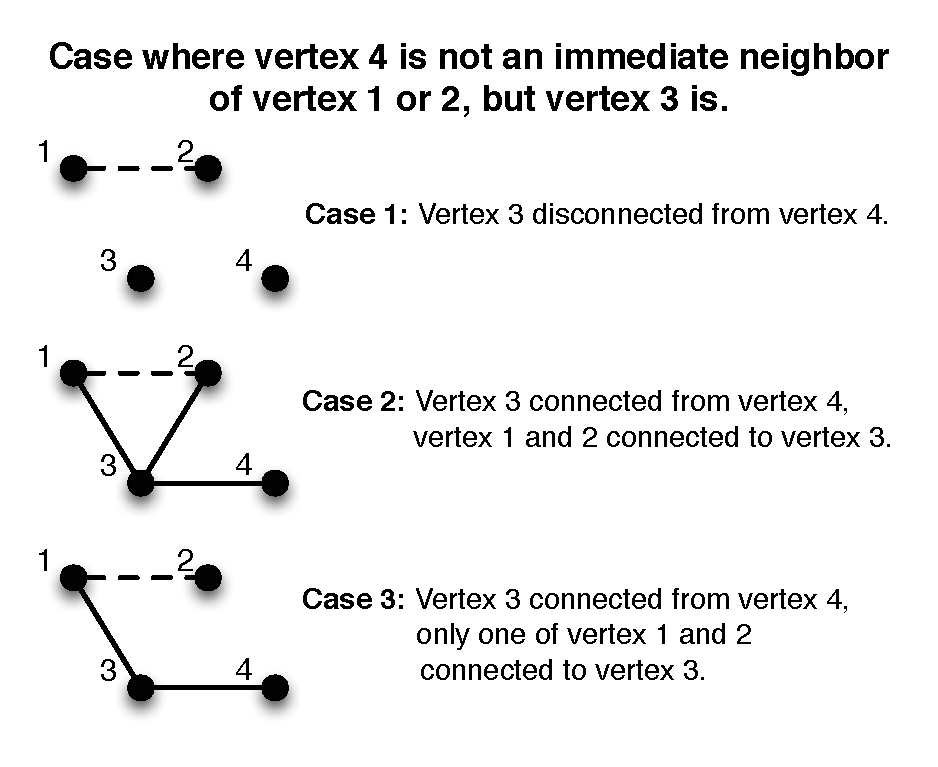
\includegraphics[width=3in]{Figures/case1.eps}
\label{fig:case}
\end{figure}

\begin{itemize}
\item Vertex $3$ is not connected to vertex $4$.  In this case, the four vertices can never form a 4-motif, regardless of whether vertices $1$ and $2$ are connected, and we don't have to change the motif counts.
\item Vertex $3$ and $4$ are connected, and vertex $1$ and $2$ are both connected to vertex $3$.  In this case, connecting vertex $1$ and $2$ deletes a four-star motif and adds a triangle-with-edge motif.
\item Vertex $3$ and $4$ are connected, and only one of vertex $1$ and $2$ are connected to vertex $3$.  In this case, connecting vertex $1$ and $2$ creates a four-line motif.
\end{itemize}

It is much faster to test for these cases than to do the normal
computations (which would involve finding the induced subgraph on those
four vertices, then testing it to see if it was either of the 4-motifs).
So implementing this optimization produces an enormous speedup, allowing us
to perform several thousand rewiring steps in one day.  Each rewiring step
is $O((d_1 + d_2)^2)$, where $d_1$ is the degree of vertex $v_1$, $d_2$
is the degree of vertex $v_2$, and $d_1 + d_2$ is an upper bound on the 
number of first-degree neighbors of $v_1$ and $v_2$.

\subsection{Random restarts}

Hill climbing is an imperfect solution since it is easy to get stuck at
local minima.  We fix this with the method of random restarts.  When we
reach a local minimum, we save the graph and begin rewiring edges randomly.
After this we run hill climbing until we reach another local minimum, then 
repeat the process.  At the end of the computation we return the graph with
lowest error.

We assume the algorithm has reached a local minimum if we have gone through
$|E|$ consecutive rewiring steps without changing the graph.  At this
point, we rewire $|E|/8$ edge pairs randomly and proceed with hill
climbing.  Preliminary results for this approach are presented in 
Section~\ref{sec:exp}.

\section{Results}
\label{sec:exp}

Hill climbing produces excellent results on most networks.  Table ~\ref{table:errors} shows the improvements in the error after running hill climbing for 24 hours.

Although performance varies across networks, we get at least a 50\% decrease in error for all networks except aut-as19990628 and cit-scimet.  For some networks we get an enormous reduction in error; pwr-power gives a 99.5\% reduction and met-HI gives a 99.9\% reduction.  The first group of figures plots the reduction in error over time and the second group plots the probability that a rewiring step will be successful (i.e. that we will accept the changes instead of discarding them).

\begin{table*}[t]
\centering
\begin{tabular}{| l | l | l | | l | l | l |}
\hline
Network & Nodes & Edges & Initial error & Final error & Successful rewires\\ \hline
aut-as19971108 & 3015 & 5156 & 0.34216 & 0.16717 & 2951.00\\\hline
aut-as19990628 & 5322 & 10163 & 0.31571 & 0.17723 & 3397.28\\\hline
cit-scimet & 3085 & 13474 & 0.83063 & 0.73247 & 1921.71\\\hline
col-ca-GrQc & 5242 & 14484 & 2.05549 & 0.93973 & 40583.8\\\hline
col-netscience & 1461 & 2742 & 3.13864 & 0.55110 & 8290.71\\\hline
met-HI & 1424 & 3423 & 8039.58 & 0.46768 & 5703.57\\\hline
ppi-ppiall & 3258 & 12930 & 1.06249 & 0.46058 & 38131.1\\\hline
ppi-ppiapms & 1622 & 9070 & 1.37580 & 0.54219 & 24581.7\\\hline
pwr-power & 4941 & 6594 & 0.57996 & 0.00282 & 9485.4\\\hline
\end{tabular}
\caption{Improvements in error after running hill climbing for 24 hours.  All numbers are averaged over $7$ trials.}
\label{table:errors}
\end{table*}

\begin{figure}[p]
\centering
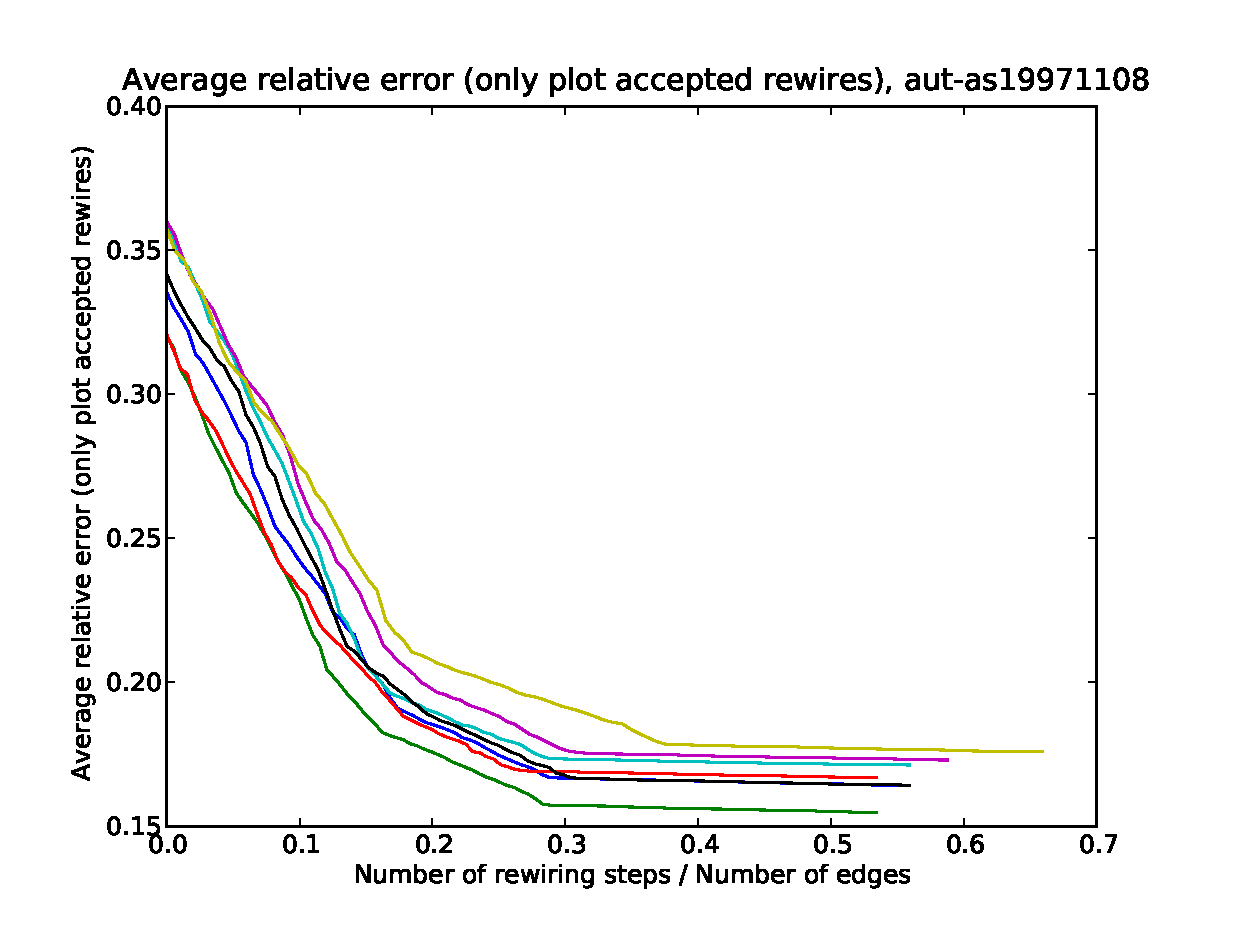
\includegraphics[width=3in]{Figures/acceptedOnly-aut-as19971108.eps}
\caption{Error, network aut-as19971108.  Only plot hill climbing steps that were successful.}
\label{fig:errors-aut-as19971108}
\end{figure}

\begin{figure}[p]
\centering
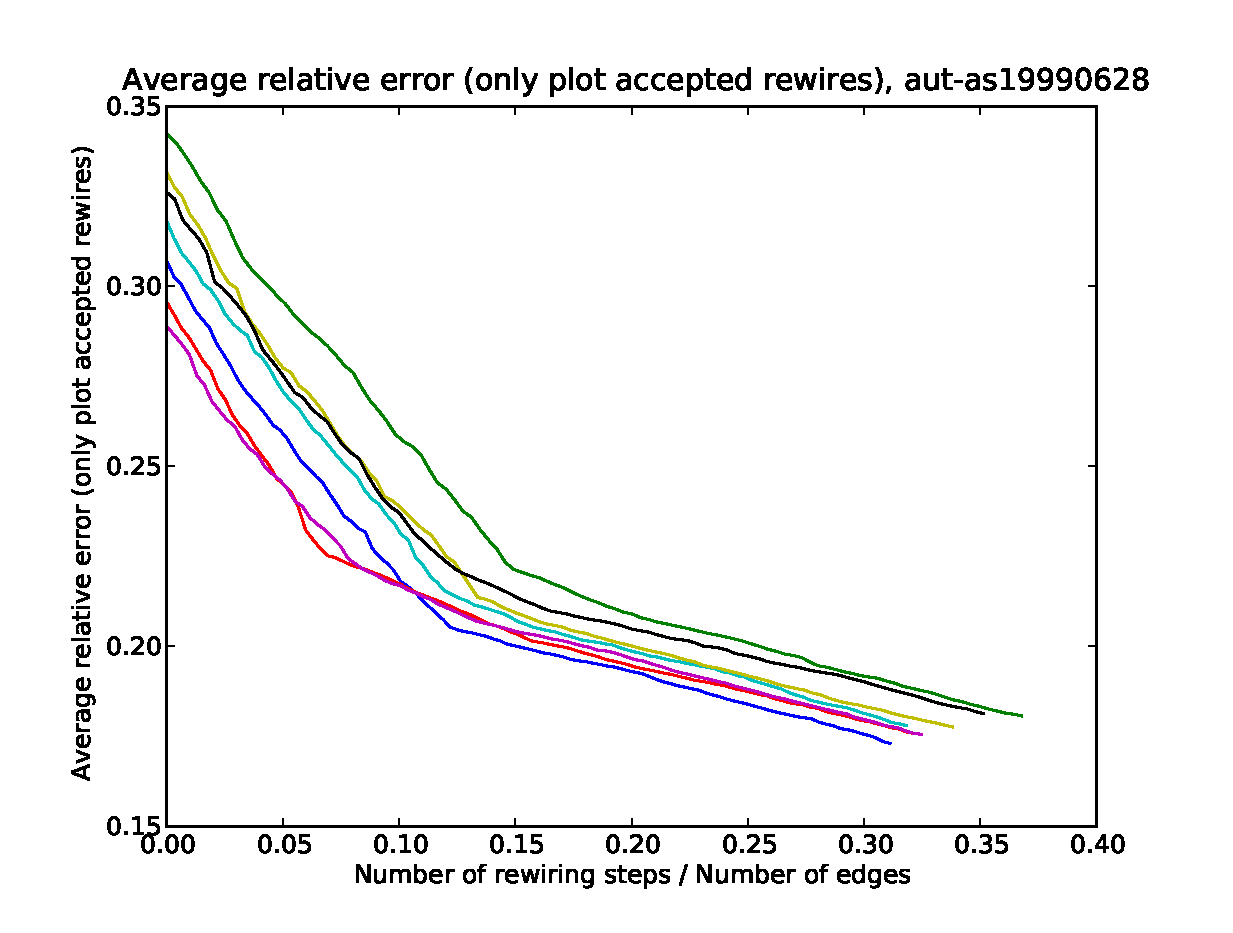
\includegraphics[width=3in]{Figures/acceptedOnly-aut-as19990628.eps}
\caption{Error, network aut-as19990628.  Only plot hill climbing steps that were successful.}
\label{fig:errors-aut-as19990628}
\end{figure}

\begin{figure}[p]
\centering
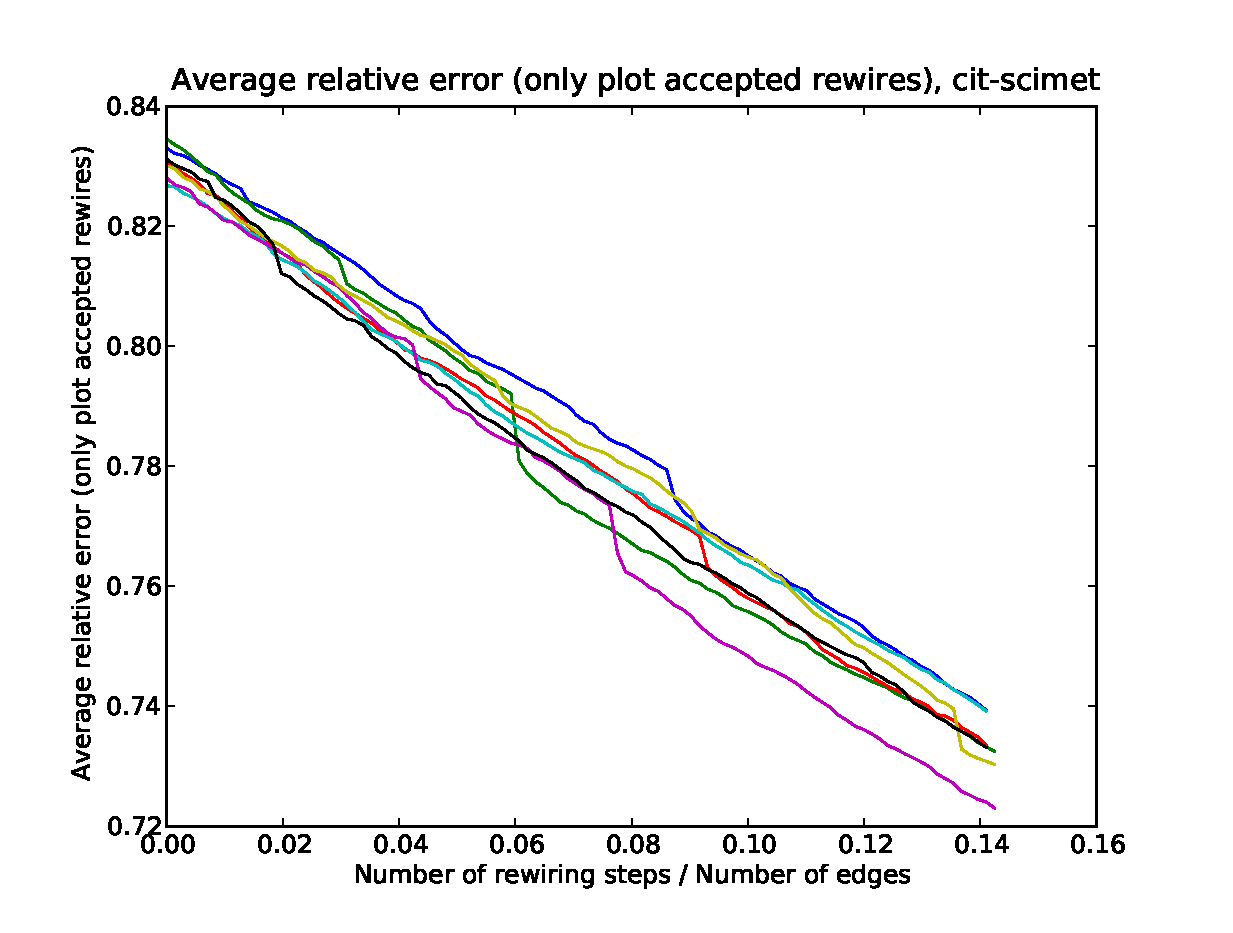
\includegraphics[width=3in]{Figures/acceptedOnly-cit-scimet.eps}
\caption{Error, network cit-scimet.  Only plot hill climbing steps that were successful.}
\label{fig:errors-cit-scimet}
\end{figure}

\begin{figure}[p]
\centering
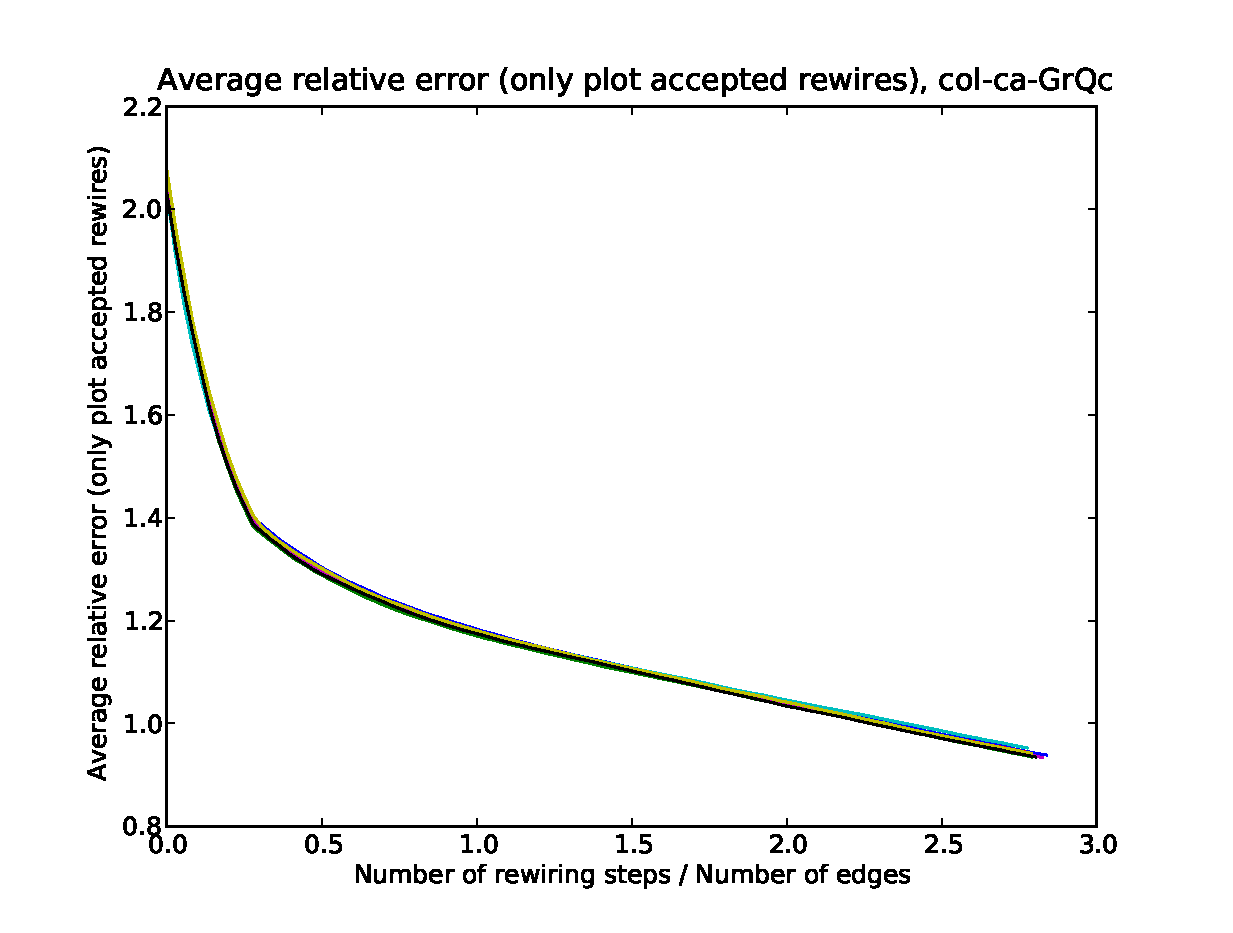
\includegraphics[width=3in]{Figures/acceptedOnly-col-ca-GrQc.eps}
\caption{Error, network col-ca-GrQc.  Only plot hill climbing steps that were successful.}
\label{fig:errors-col-ca-GrQc}
\end{figure}

\begin{figure}[p]
\centering
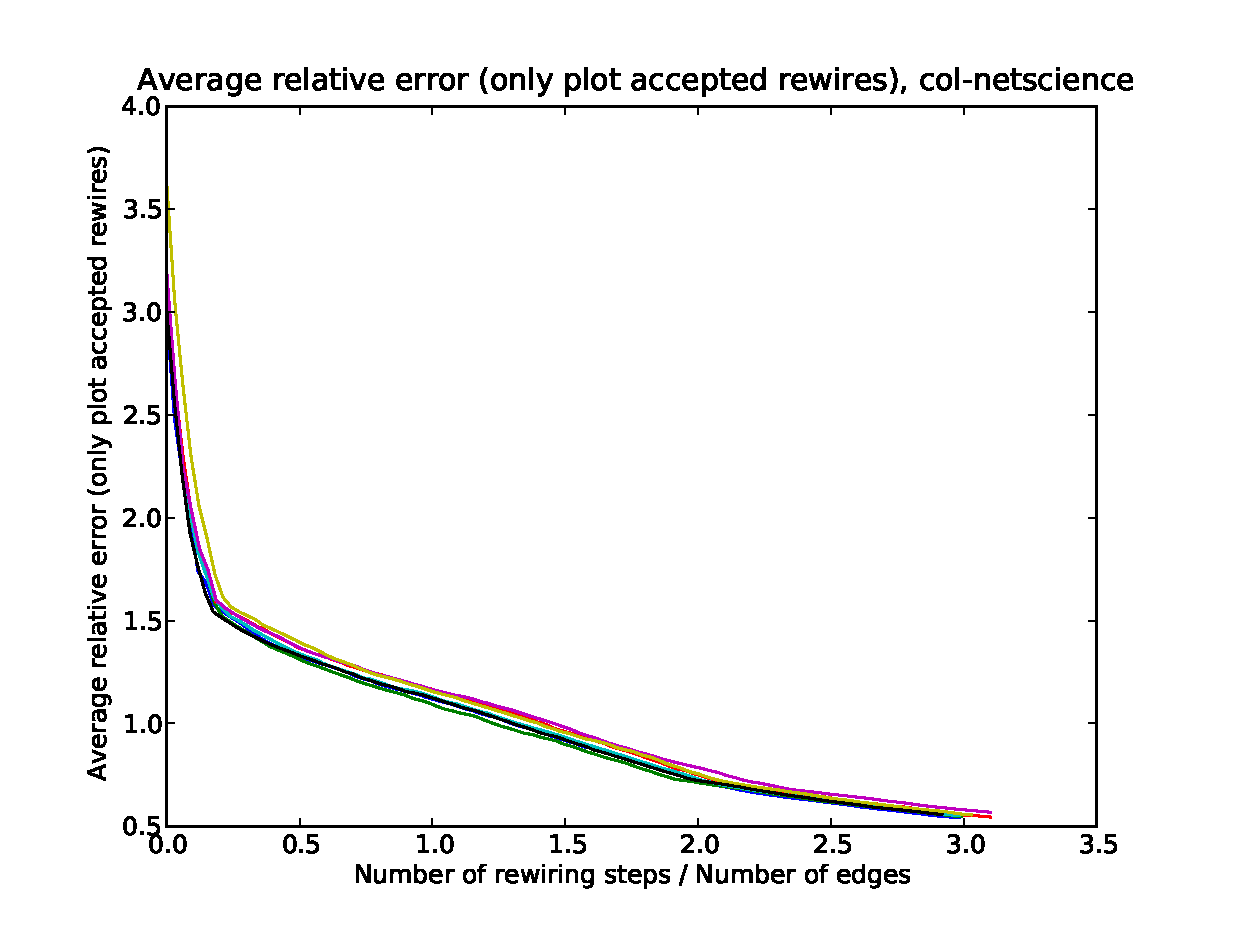
\includegraphics[width=3in]{Figures/acceptedOnly-col-netscience.eps}
\caption{Error, network col-netscience.  Only plot hill climbing steps that were successful.}
\label{fig:errors-col-netscience}
\end{figure}

\begin{figure}[p]
\centering
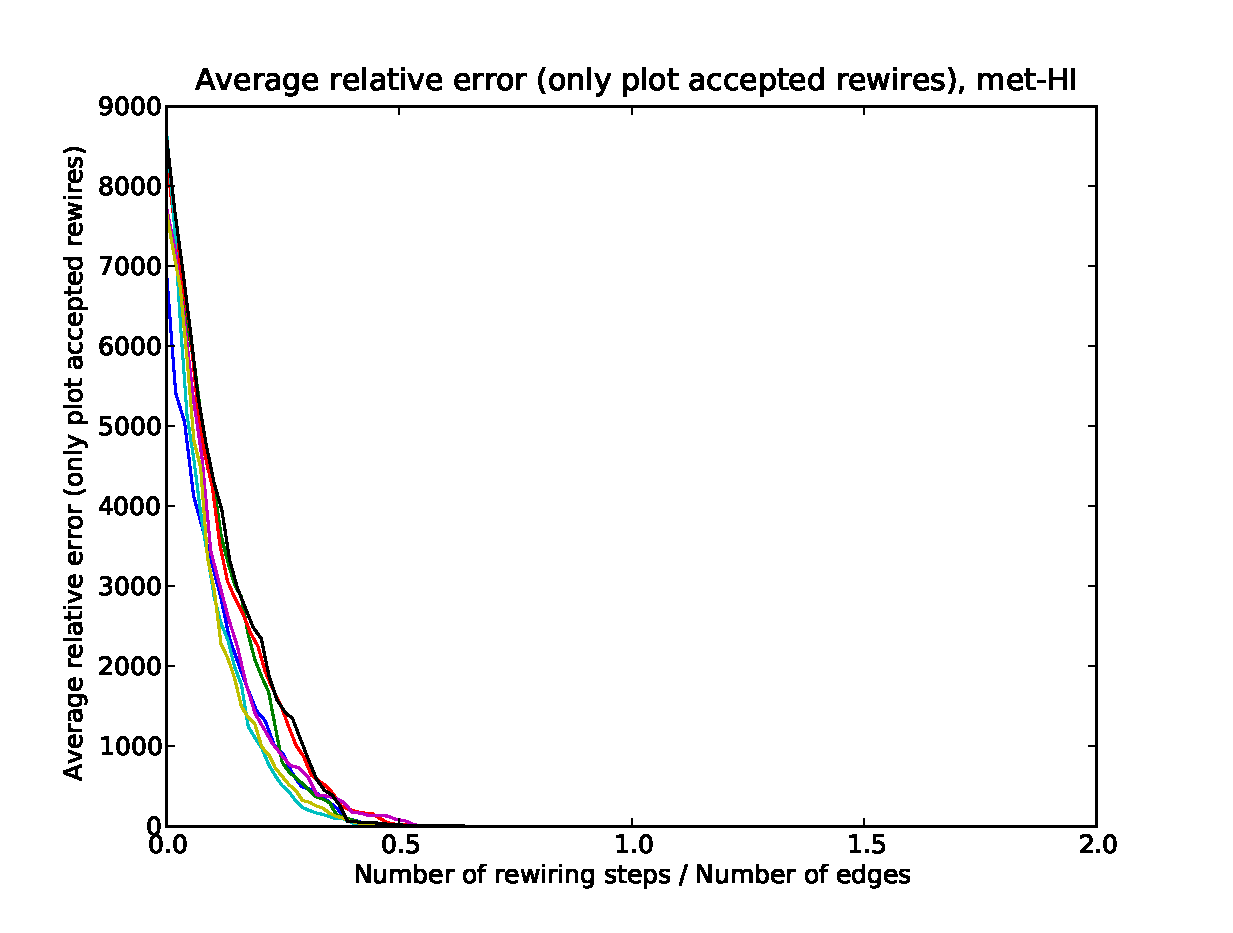
\includegraphics[width=3in]{Figures/acceptedOnly-met-HI.eps}
\caption{Error, network met-HI.  Only plot hill climbing steps that were successful.}
\label{fig:errors-met-HI}
\end{figure}

\begin{figure}[p]
\centering
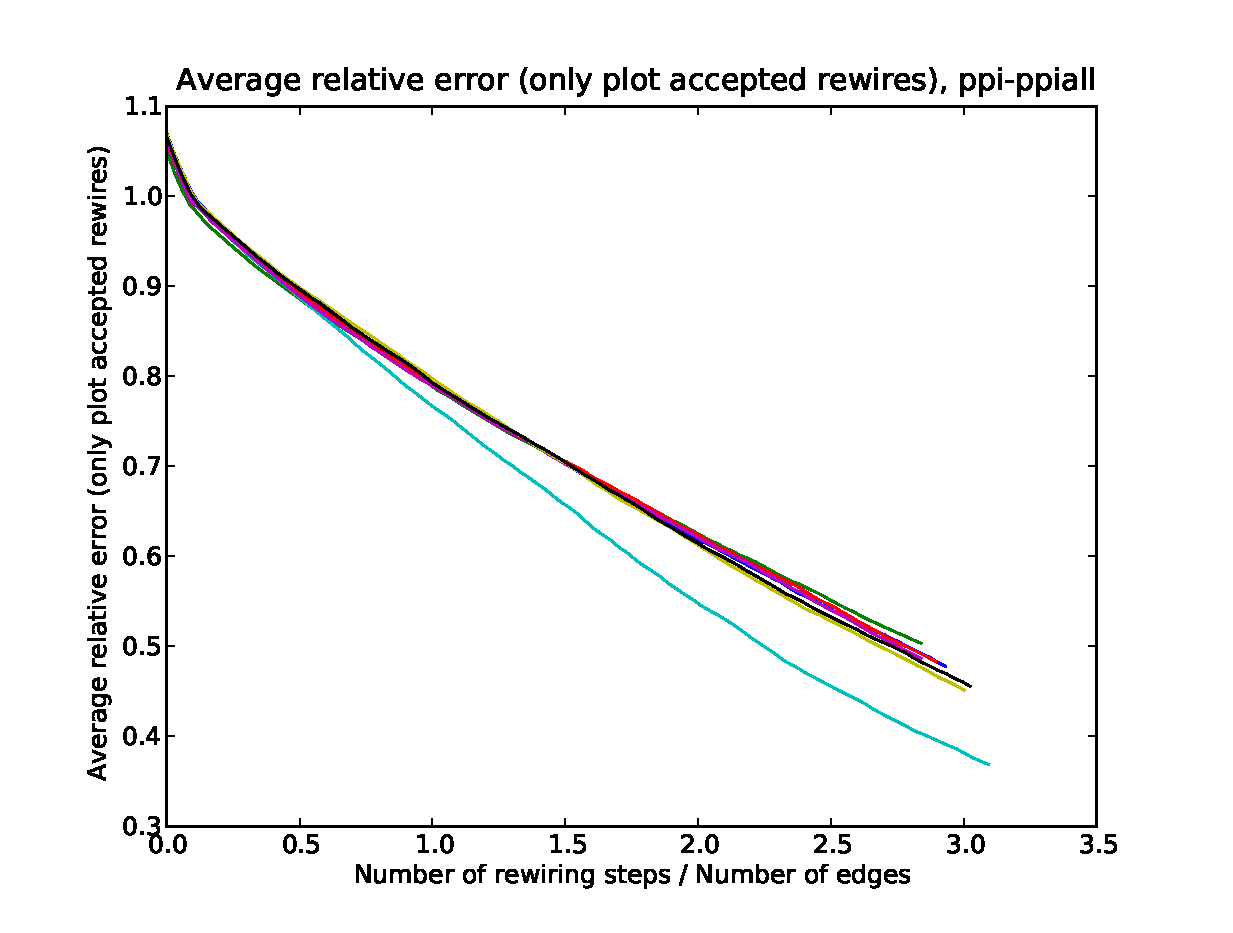
\includegraphics[width=3in]{Figures/acceptedOnly-ppi-ppiall.eps}
\caption{Error, network ppi-ppiall.  Only plot hill climbing steps that were successful.}
\label{fig:errors-ppi-ppiall}
\end{figure}

\begin{figure}[p]
\centering
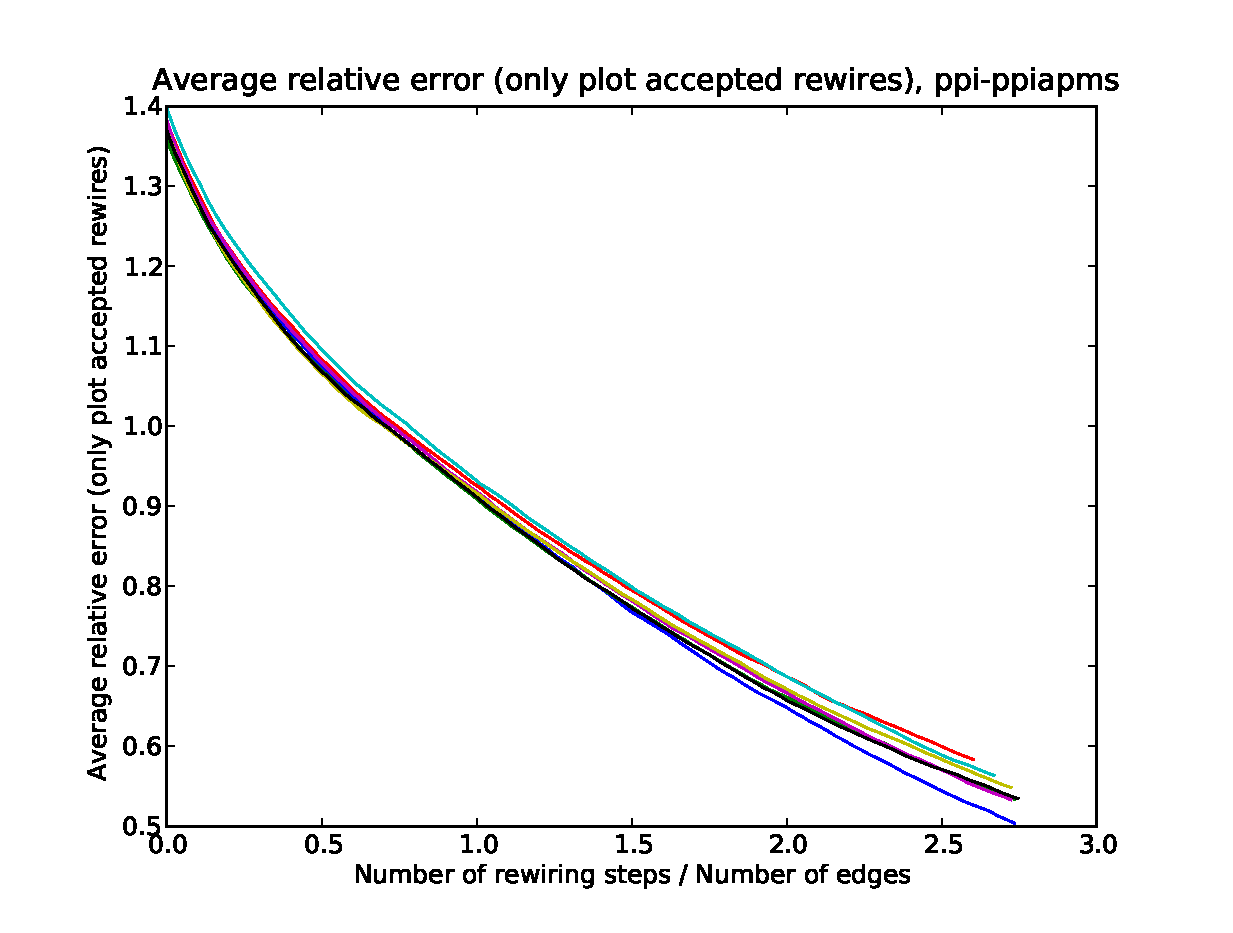
\includegraphics[width=3in]{Figures/acceptedOnly-ppi-ppiapms.eps}
\caption{Error, network ppi-ppiapms.  Only plot hill climbing steps that were successful.}
\label{fig:errors-ppi-ppiapms}
\end{figure}

\begin{figure}[p]
\centering
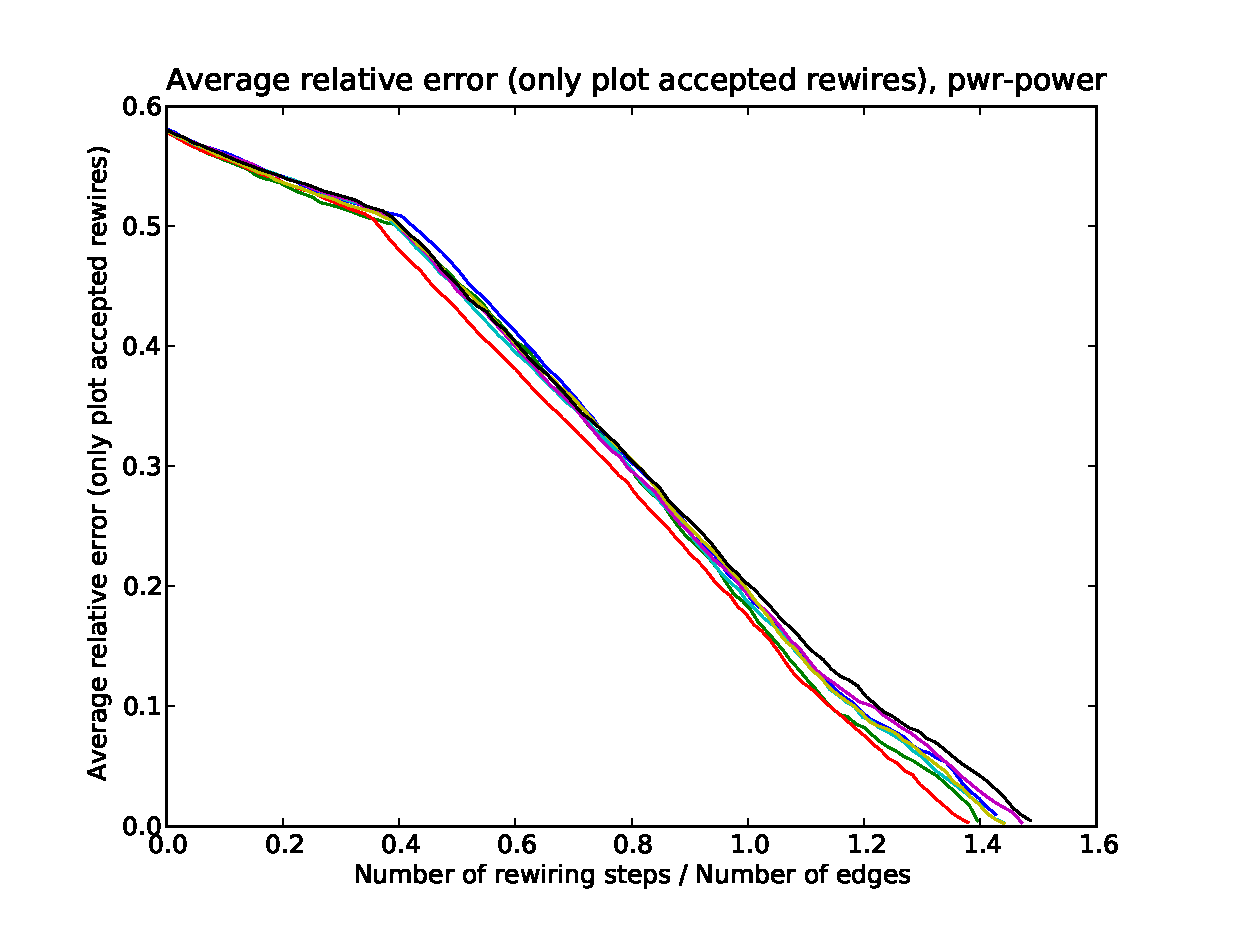
\includegraphics[width=3in]{Figures/acceptedOnly-pwr-power.eps}
\caption{Error, network pwr-power.  Only plot hill climbing steps that were successful.}
\label{fig:errors-pwr-power}
\end{figure}

\begin{figure}[p]
\centering
\includegraphics[width=3in]{Figures/Paccept-aut-as19971108.eps}
\caption{Probability of a rewiring step being successful, network aut-as19971108}
\label{fig:Paccept-aut-as19971108}
\end{figure}

\begin{figure}[p]
\centering
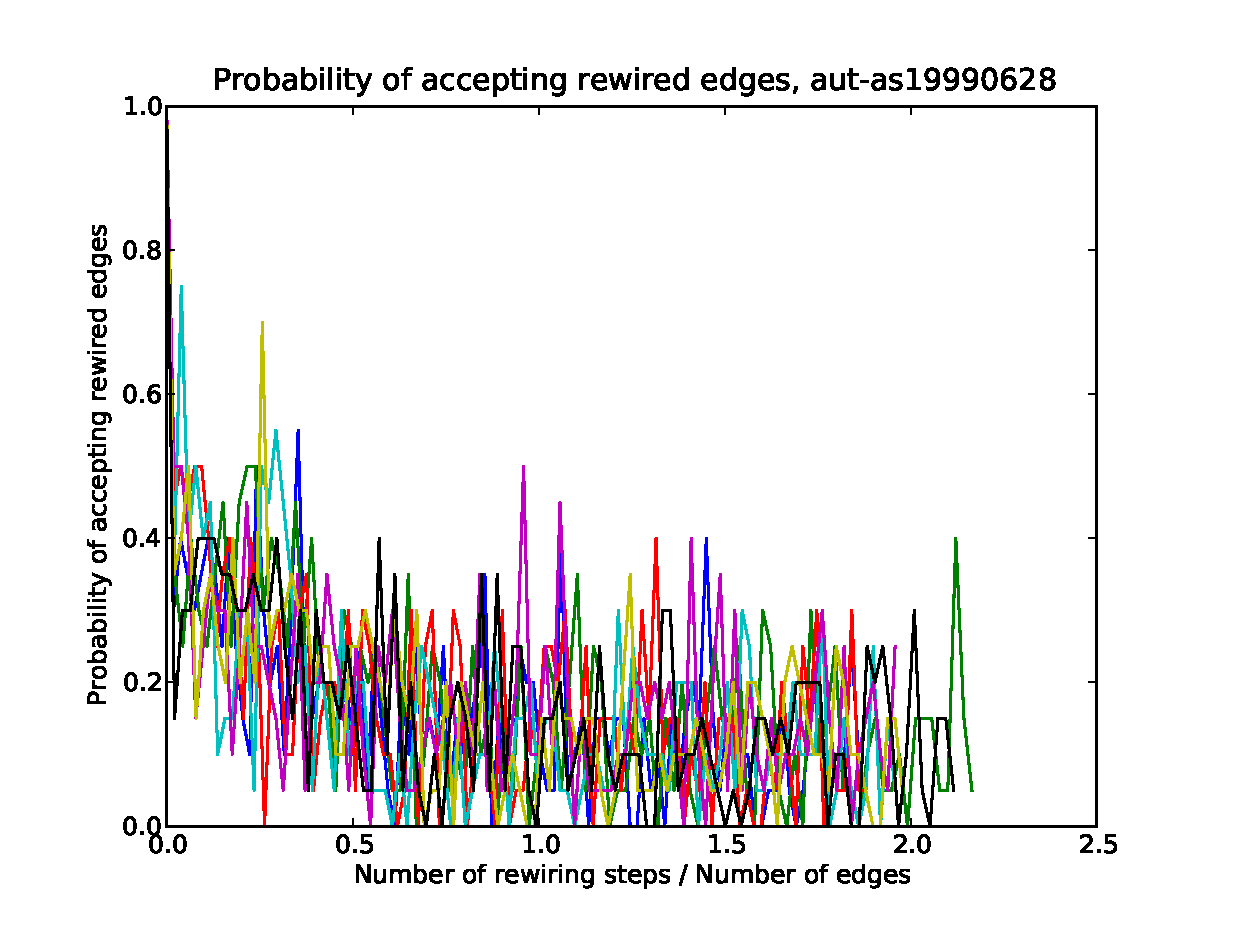
\includegraphics[width=3in]{Figures/Paccept-aut-as19990628.eps}
\caption{Probability of a rewiring step being successful, network aut-as19990628}
\label{fig:Paccept-aut-as19990628}
\end{figure}

\begin{figure}[p]
\centering
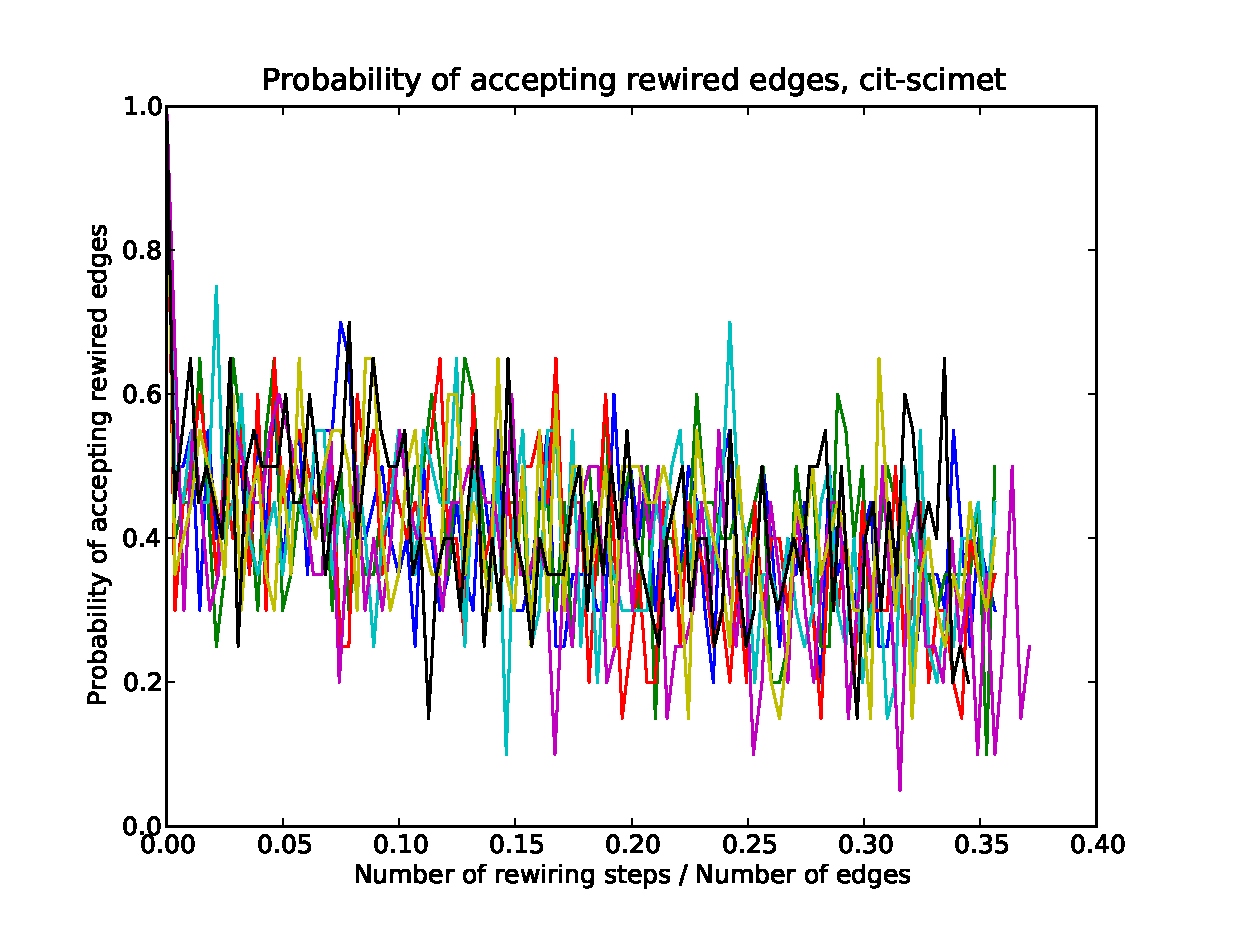
\includegraphics[width=3in]{Figures/Paccept-cit-scimet.eps}
\caption{Probability of a rewiring step being successful, network cit-scimet}
\label{fig:Paccept-cit-scimet}
\end{figure}

\begin{figure}[p]
\centering
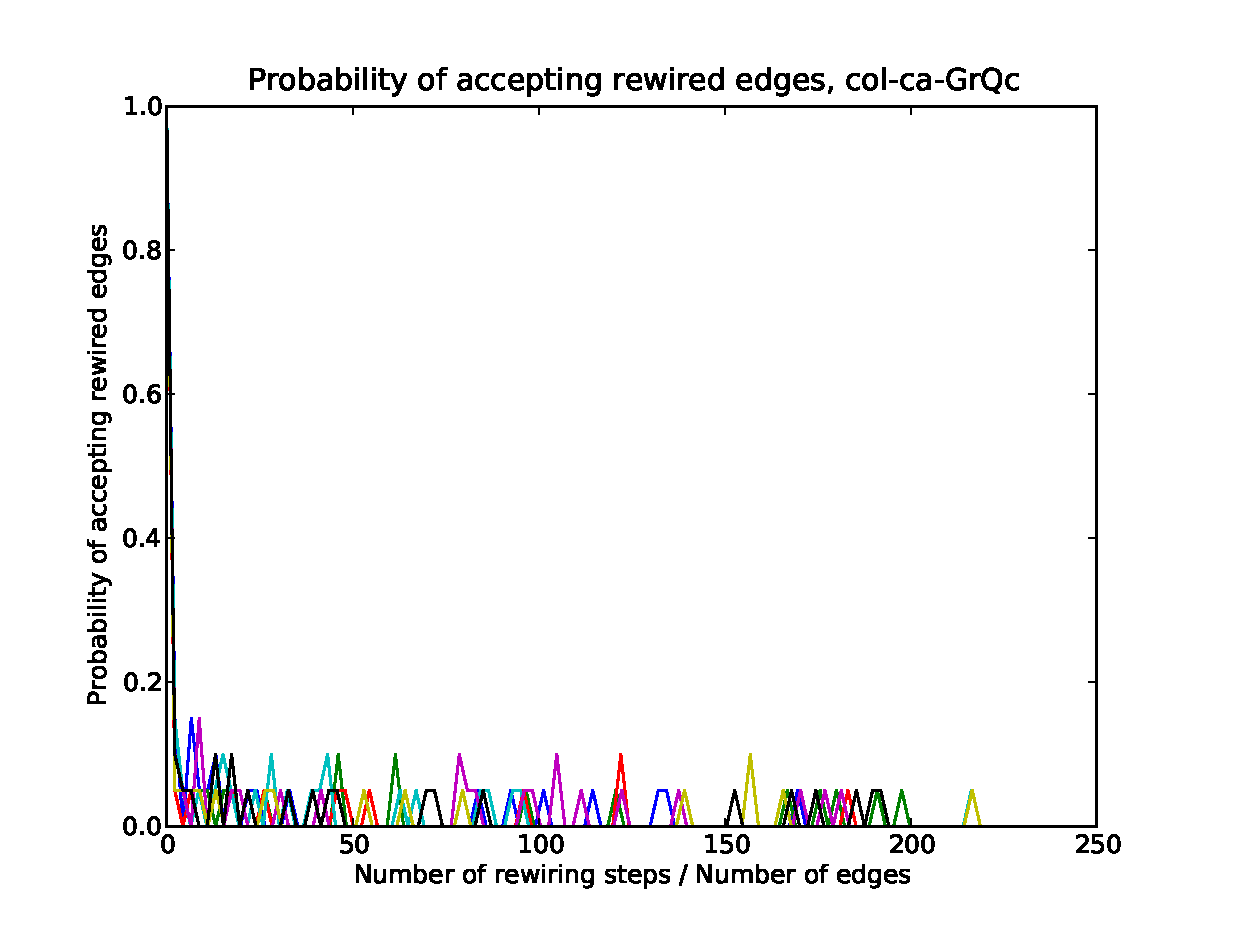
\includegraphics[width=3in]{Figures/Paccept-col-ca-GrQc.eps}
\caption{Probability of a rewiring step being successful, network col-ca-GrQc}
\label{fig:Paccept-col-ca-GrQc}
\end{figure}

\begin{figure}[p]
\centering
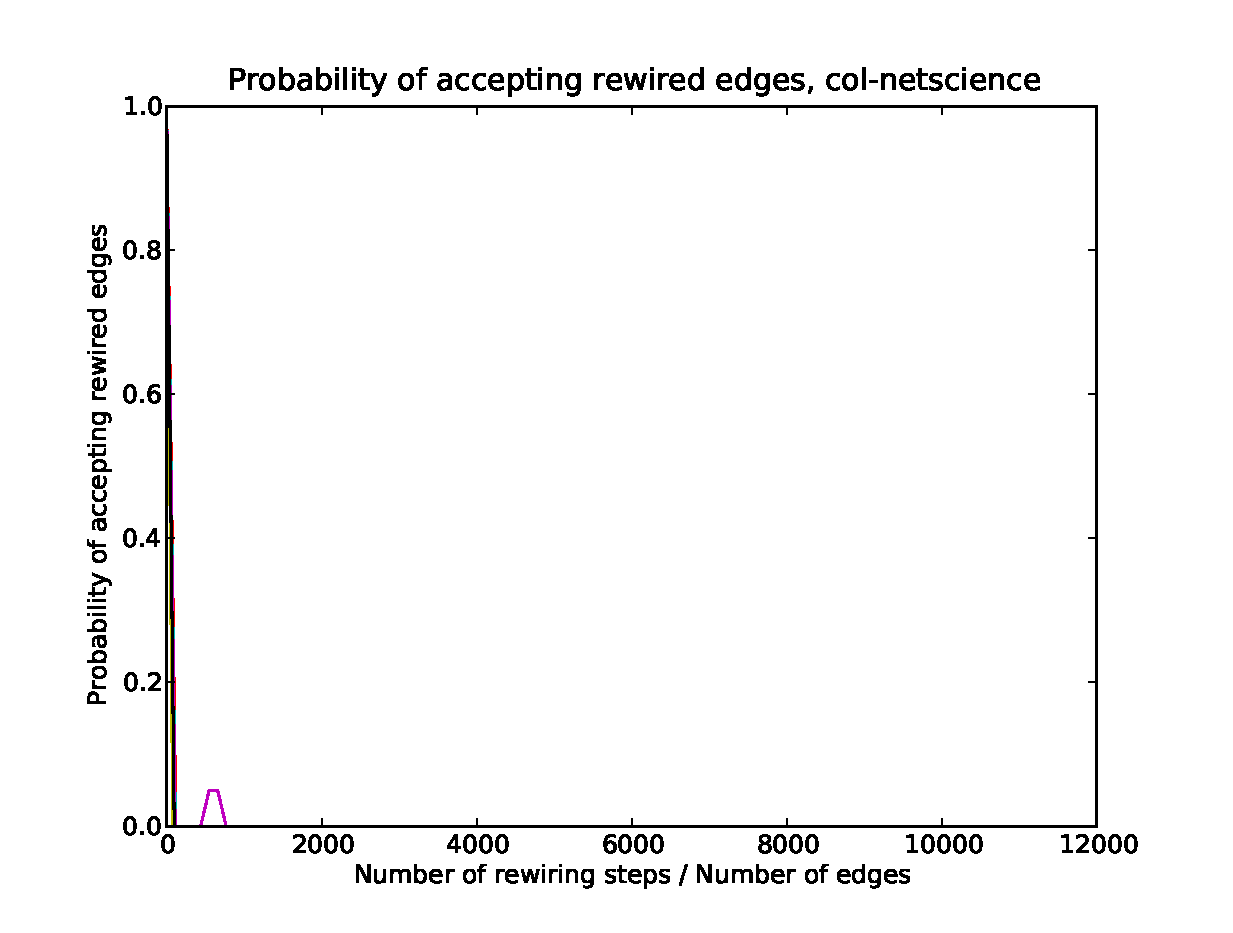
\includegraphics[width=3in]{Figures/Paccept-col-netscience.eps}
\caption{Probability of a rewiring step being successful, network col-netscience}
\label{fig:Paccept-col-netscience}
\end{figure}

\begin{figure}[p]
\centering
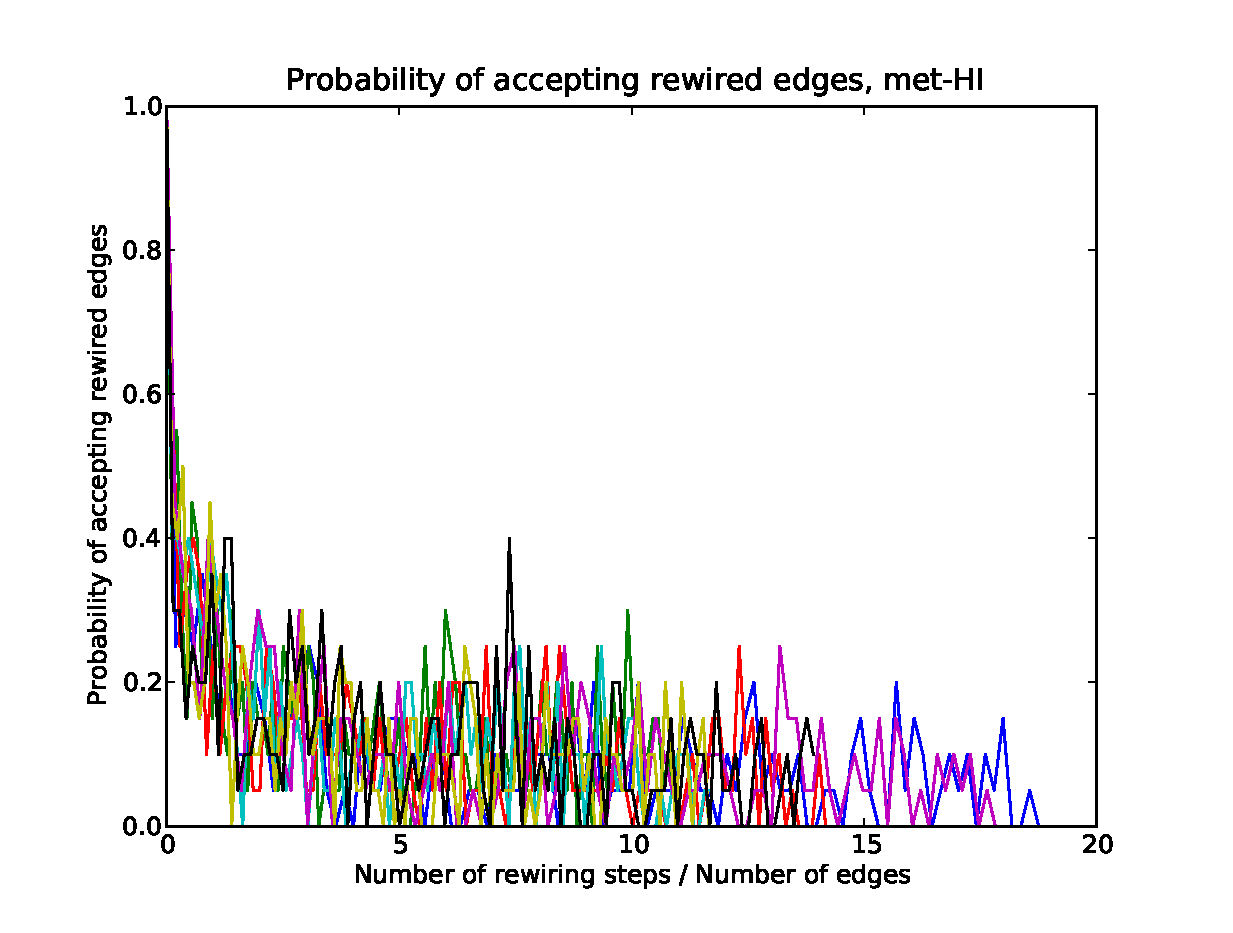
\includegraphics[width=3in]{Figures/Paccept-met-HI.eps}
\caption{Probability of a rewiring step being successful, network met-HI}
\label{fig:Paccept-met-HI}
\end{figure}

\begin{figure}[p]
\centering
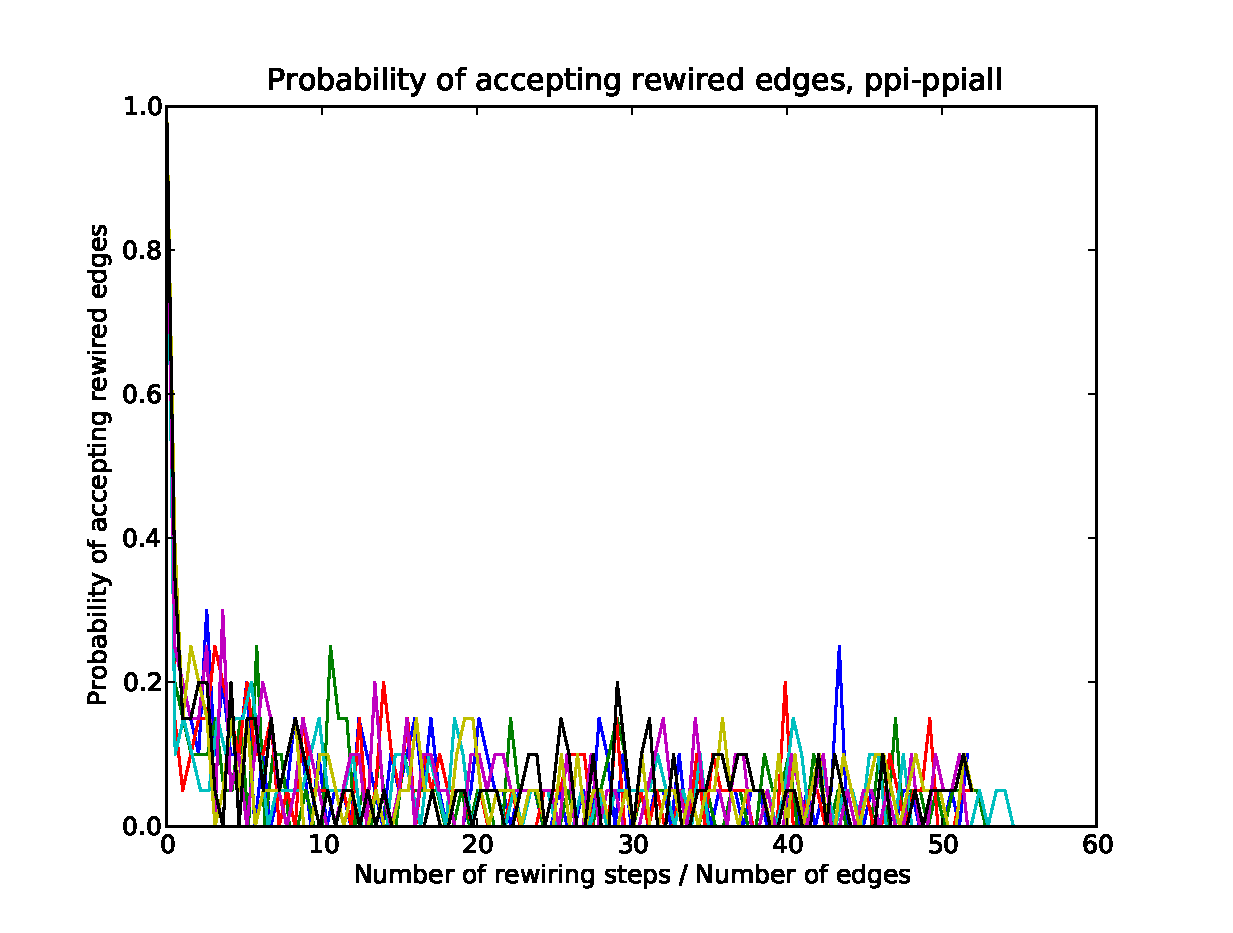
\includegraphics[width=3in]{Figures/Paccept-ppi-ppiall.eps}
\caption{Probability of a rewiring step being successful, network ppi-ppiall}
\label{fig:Paccept-ppi-ppiall}
\end{figure}

\begin{figure}[p]
\centering
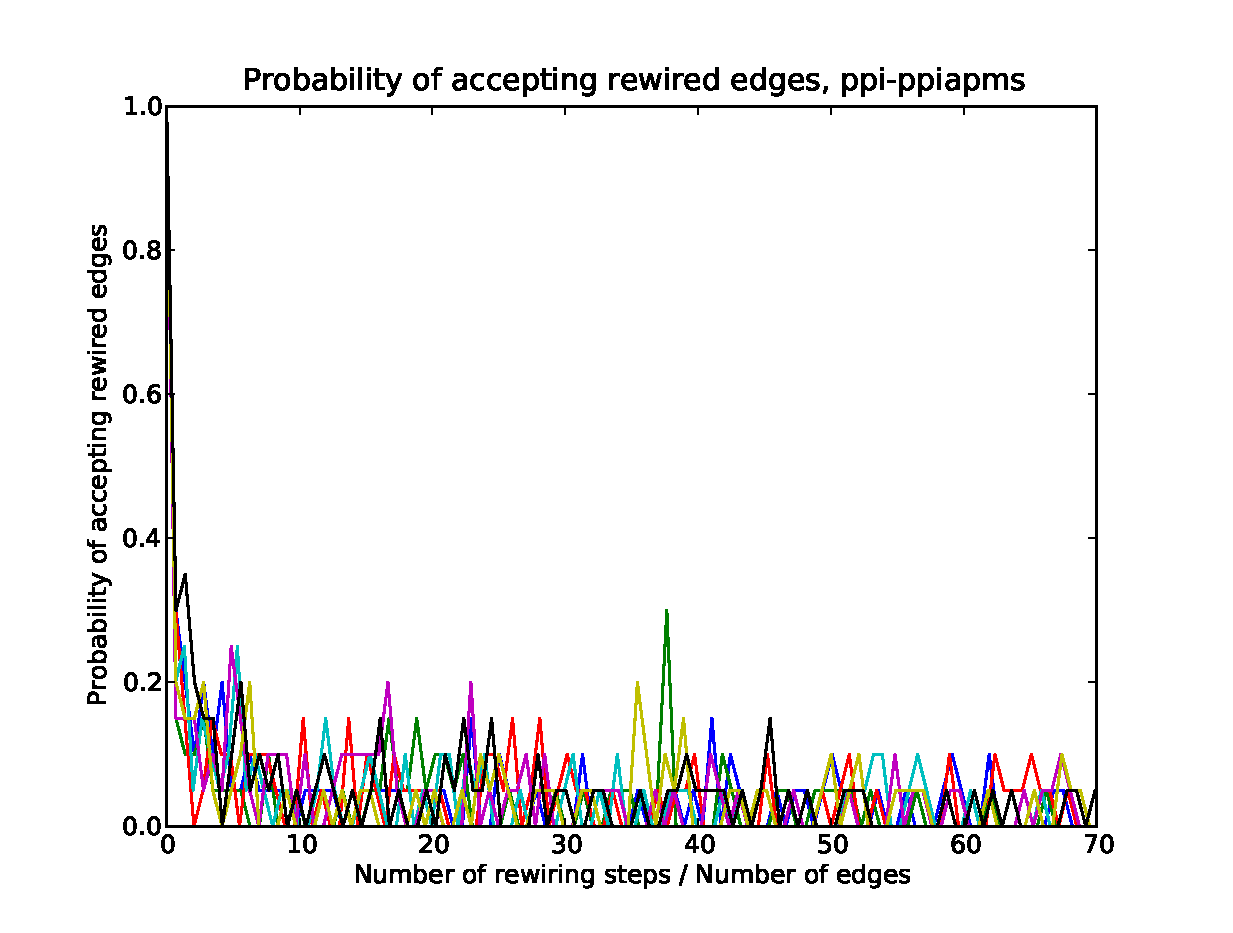
\includegraphics[width=3in]{Figures/Paccept-ppi-ppiapms.eps}
\caption{Probability of a rewiring step being successful, network ppi-ppiapms}
\label{fig:Paccept-ppi-ppiapms}
\end{figure}

\begin{figure}[p]
\centering
\includegraphics[width=3in]{Figures/Paccept-pwr-power.eps}
\caption{Probability of a rewiring step being successful, network pwr-power}
\label{fig:Paccept-pwr-power}
\end{figure}
\section{Future work}
\label{sec:related}

Our current algorithms assume that we know the degree distribution of the graph.  This is fine if we have the graph of a real-world social network and we are trying to build a model to compare it to.  However, it fails if we are given the motif counts only.

Fortunately, social networks tend to have power-law degree distributions, which means their distributions can be described by a single parameter $\alpha$, where $\alpha$ is the magnitude of the exponent.  (We also need a normalization constant, which can be found from the number of edges.)  For the final paper we will build a model to predict $\alpha$ from the motif counts.  We think we can do this because graphs with a lot of high-edge motifs should be denser, so the degree distribution should have a heavier tail.

Models to try include linear regression, neural networks, and stochastic gradient descent.
\input{conclusion.tex}

\bibliographystyle{abbrv}
\bibliography{references}  % sigproc.bib is the name of the Bibliography in this case

%\input{appendix.tex}

\end{document}

